\documentclass{article}
\usepackage{graphicx}
\graphicspath{ {./images/} }
\usepackage{amsmath}

\title{2. Gausa metode. Determinanti.}
\author{Gunārs Ābeltiņš}
\date{2022.03.07}

\begin{document}

\maketitle

\section*{Lekcijas konspekts}
Tika stāstīts par determinanta īpašībām. Parādija kā to aprēķināt. Kramera formulas.

\clearpage

\section*{1. Uzdevums}
Aprēķiniet determinantu $Det[\{6,5,7\},\{4,3,1\},\{3,2,3\}]$, izmantojot lekcijā doto 3x3 determinanta definīciju (ne savādāk). Parādiet katru aprēķina soli. Rezultātu pārbaudiet ar WolframAlpha.

\begin{gather*}
    \det
    \begin{pmatrix}
        6 & 5 & 7\\
        4 & 3 & 1\\
        3 & 2 & 3
    \end{pmatrix} 
    =
    \begin{vmatrix}
        6 & 5 & 7\\
        4 & 3 & 1\\
        3 & 2 & 3
    \end{vmatrix}
    =
    6 \begin{vmatrix} 3 & 1 \\ 2 & 3 \end{vmatrix} 
    - 5 \begin{vmatrix} 4 & 1 \\ 3 & 3 \end{vmatrix} 
    + 7 \begin{vmatrix} 4 & 3 \\ 3 & 2 \end{vmatrix}
    =
    \\
    =
    6 \det\begin{pmatrix} 3 & 1 \\ 2 & 3 \end{pmatrix} 
    - 5 \det\begin{pmatrix} 4 & 1 \\ 3 & 3 \end{pmatrix} 
    + 7 \det\begin{pmatrix} 4 & 3 \\ 3 & 2 \end{pmatrix}
    =
    \\
    =
    6((3 \cdot 3) - (1 \cdot 2)) 
    - 5((4 \cdot 3) - (1 \cdot 3)) 
    + 7((4 \cdot 2) - (3 \cdot 3))
    =
    \\
    =
    6 \cdot 7 - 5 \cdot 9 + 7 \cdot (-1)
    =
    42 - 45 - 7
    =
    (-10)
\end{gather*}

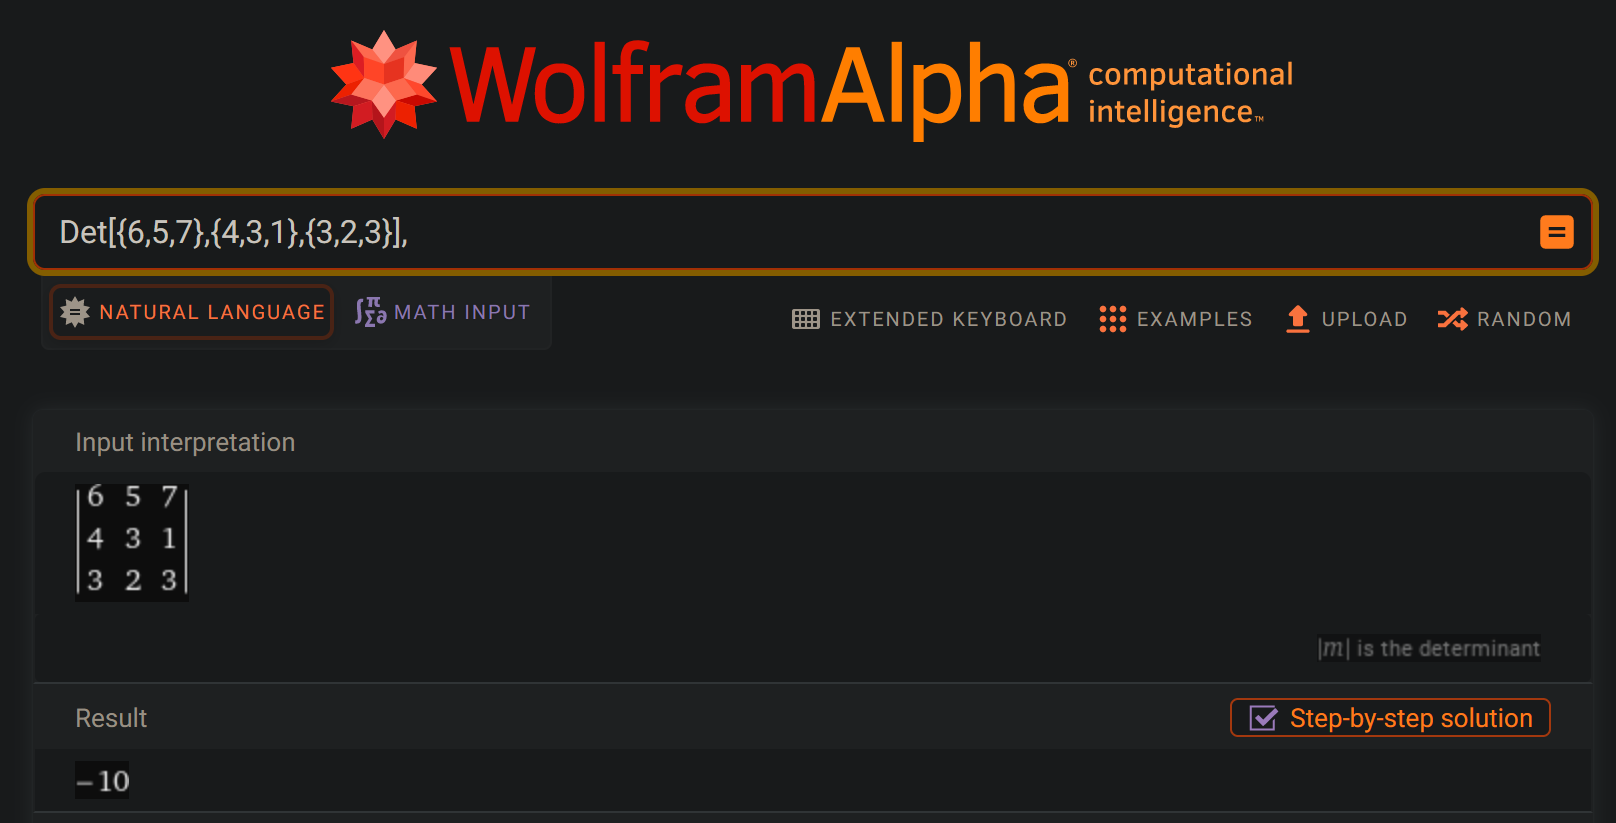
\includegraphics[width=\textwidth]{1}

\clearpage

\section*{2. Uzdevums}
Izmantojiet Kramera formulas, lai atrisinātu vienādojumu sistēmu \{2x-7y+2z=9, 3x+2y+2z=8, 4x+5y+2z=4\}. Vajadzīgos determinantus uzrakstiet, bet aprēķiniet ar WolframAlpha. Risinājuma pareizību pārbaudiet ar WolframAlpha.

\begin{equation*}
    \begin{cases}
        2x - 7y + 2z = 9\\
        3x + 2y + 2z = 8\\
        4x + 5y + 2z = 4\\
    \end{cases}
\end{equation*}

\begin{equation*}
    x
    = 
    \frac
    {
        \det
        \begin{pmatrix}
            9 & -7 & 2\\
            8 & 2 & 2\\
            4 & 5 & 2
        \end{pmatrix}
    }
    {
        \det
        \begin{pmatrix}
            2 & -7 & 2\\
            3 & 2 & 2\\
            4 & 5 & 2
        \end{pmatrix}
    }
    =
    \frac{66}{-12}
    =
    - \frac{11}{2}
\end{equation*}

\begin{equation*}
    y
    = 
    \frac
    {
        \det
        \begin{pmatrix}
            2 & 9 & 2\\
            3 & 8 & 2\\
            4 & 4 & 2
        \end{pmatrix}
    }
    {
        \det
        \begin{pmatrix}
            2 & -7 & 2\\
            3 & 2 & 2\\
            4 & 5 & 2
        \end{pmatrix}
    }
    =
    \frac{-6}{-12}
    =
    0.5
\end{equation*}

\begin{equation*}
    z
    = 
    \frac
    {
        \det
        \begin{pmatrix}
            2 & -7 & 9\\
            3 & 2 & 8\\
            4 & 5 & 4
        \end{pmatrix}
    }
    {
        \det
        \begin{pmatrix}
            2 & -7 & 2\\
            3 & 2 & 2\\
            4 & 5 & 2
        \end{pmatrix}
    }
    =
    \frac{-141}{-12}
    =
    \frac{47}{4}
\end{equation*}

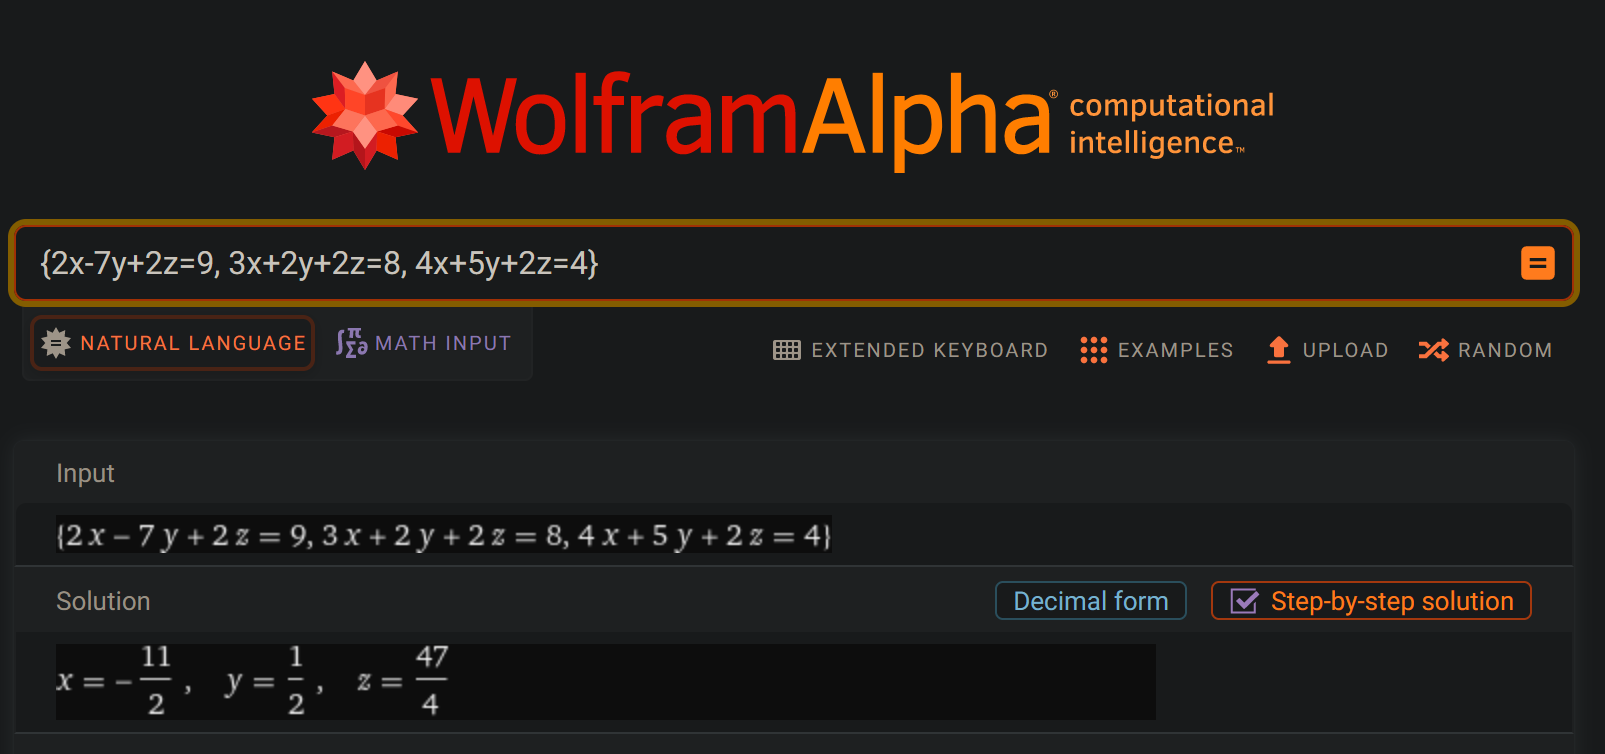
\includegraphics[width=\textwidth]{2}

\clearpage

\section*{3. Uzdevums}
Izgudrojiet un uzrakstiet 3x3 determinantu piemērus, kas parādītu, kā Jūs saprotat determinantu īpašības 6, 7, 8. Nepieciešamos determinantus aprēķiniet ar WolframAlpha.

\subsection*{6. Īpašība}
Ja matricā kāda rinda ir iegūta no citas rindas, reizinot ar kādu skaitli (t.i. divas rindas ir proporcionālas), tad matricas determinanta vērtība ir 0.
\begin{equation*}
    \begin{vmatrix}
        1 & (2 \cdot 1) & 11\\
        2 & (2 \cdot 2) & 13\\
        3 & (2 \cdot 3) & 17
    \end{vmatrix}
    =
    \begin{vmatrix}
        1 & 2 & 11\\
        2 & 4 & 13\\
        3 & 6 & 17
    \end{vmatrix}
    =
    0
\end{equation*}

\subsection*{7. Īpašība}
Ja matricas A i-jā rindā katrs elements ir divu skaitļu summa $a_{ij}=b_{j}+c_{j}$, tad $det(A)=det(B)+det(C)$, kur matricas B un C ir iegūtas no A, aizstājot i-jā rindā katru $a_{ij}$ attiecīgi ar $b_{j}$ vai $c_{j}$.
\begin{equation*}
    \begin{vmatrix}
        1 & 6 & 11\\
        2 & 4 & 13\\
        3 & 2 & 17
    \end{vmatrix}
    =
    16
\end{equation*}
\begin{equation*}
    \begin{vmatrix}
        1 & 6 & (4 + 7)\\
        2 & 4 & (10 + 3)\\
        3 & 2 & (7 + 10)
    \end{vmatrix}
    =
    \begin{vmatrix}
        1 & 6 & 4\\
        2 & 4 & 10\\
        3 & 2 & 7
    \end{vmatrix}
    +
    \begin{vmatrix}
        1 & 6 & 7\\
        2 & 4 & 3\\
        3 & 2 & 10
    \end{vmatrix}
    =
    72 + (-88)
    =
    16
\end{equation*}

\subsection*{8. Īpašība}
Ja determinantā kādai rindai pieskaita vai atņem citu rindu, pareizinātu ar kādu skaitli, tad determinanta vērtība nemainās
\begin{equation*}
    \begin{vmatrix}
        1 & 6 & 4\\
        2 & 4 & 10\\
        3 & 2 & 7
    \end{vmatrix}
    =
    72
\end{equation*}
\begin{equation*}
    \begin{vmatrix}
        1 & 6 & 4\\
        2 & 4 & 10\\
        3 & 2 & 7
    \end{vmatrix}
    =
    \begin{vmatrix}
        1 & (6 + 1) & 4\\
        2 & (4 + 2) & 10\\
        3 & (2 + 3) & 7
    \end{vmatrix}
    =
    \begin{vmatrix}
        1 & 7 & 4\\
        2 & 6 & 10\\
        3 & 5 & 7
    \end{vmatrix}
    =
    72
\end{equation*}

\end{document}
